\documentclass{bredelebeamer}


\begin{document}

\title[PBRS for MARL]{\textbf{Plan-Based Reward Shaping for Multi-Agent Reinforcement Learning} \\INFO-F-409 -- Learning dynamics} % The short title appears at the bottom of every slide, the full title is only on the title page

\author[]{Jérome \textsc{Bastogne}, Maxime \textsc{Desclefs}, Simon \textsc{Picard}}
\institute[ULB] % Your institution as it will appear on the bottom of every slide, may be shorthand to save space
{
Université Libre de Bruxelles, Boulevard du Triomphe - CP 212, 1050 Brussels, Belgium \\ % Your institution for the title page
\medskip
\textit{jbastogn@ulb.ac.be, mdesclef@ulb.ac.be, spicard@ulb.ac.be} % Your email address
}
\date{January 15 2016} % Date, can be changed to a custom date

\begin{frame}
\titlepage % Print the title page as the first slide
\end{frame}

\begin{frame}{Content}
\tableofcontents % Throughout your presentation, if you choose to use \section{} and \subsection{} commands, these will automatically be printed on this slide as an overview of your presentation
\end{frame}

\section{Introduction}
\begin{frame}{Introduction}

\begin{block}{}
\begin{itemize}
\item Reinforcement learning
\item Increase speed through prior knowledge
\item Multi-agent
\item Plan
\end{itemize}
\end{block}

\end{frame}

\section{Materials and Methods}
\subsection{Reinforcement Learning}
\begin{frame}{Reinforcement Learning}

\begin{block}{Q-Matrix}
\begin{itemize}
\item MDP =  $< S, A, T, R >$
\item $Q(s, a) \leftarrow  Q(s, a) +  \alpha [r + \gamma Q(s', a') - Q(s,a)]$
\item $\alpha$ : learning rate
\item $r$ : reward
\item $\gamma$ : discount factor
\end{itemize}
\end{block}

\begin{block}{Eligibility traces}
\begin{itemize}
\item $Q(s, a) \leftarrow  Q(s, a) +  \alpha *  \sigma *  (\gamma * \lambda)^t$
\item $\sigma = r + \gamma Q(s', a') - Q(s,a)$
\item $\lambda$ : eligibility factor
\end{itemize}
\end{block}

\end{frame}


\subsection{Plan Based Reward Shaping}
\begin{frame}{Reward Shaping}

\begin{block}{Basic}
\begin{itemize}
\item $Q(s, a) \leftarrow  Q(s, a) +  \alpha [r + F(s, s') + \gamma Q(s', a') - Q(s,a)]$
\item $F(s, s') =\gamma \phi (s') - \phi (s)$
\item Potential function over a state
\end{itemize}
\end{block}

\begin{columns}

\begin{column}{0.7\linewidth}

\begin{block}{Plan Based Reward Shaping}
\begin{itemize}
\item Set of subgoals
\item To be followed in order
\item Proportional to the step in the plan
\end{itemize}
\end{block}

\end{column}

\begin{column}{0.3\linewidth}

\begin{figure}[h!]
\centering
  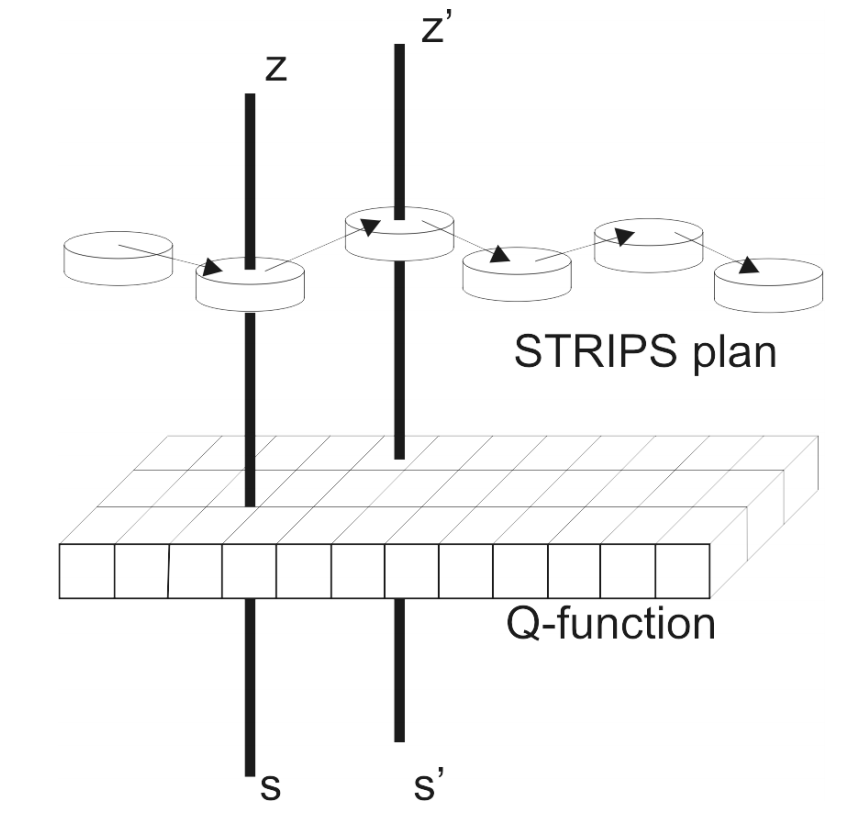
\includegraphics[width = \linewidth]{../article/img/strips.png}
  \caption{Plan-base reward shaping}
  \label{fig:strips}
\end{figure}

\end{column}

\end{columns}

\end{frame}


\begin{frame}

\begin{block}{Multi-Agent Planning}
\begin{itemize}
\item How to set the plan
\item Information sharing
\item One centralized agent : joint plans
\item Each agent make its plan : individual plans
\end{itemize}
\end{block}

\begin{block}{Multi-Agent, Plan-Based Reward Shaping}
\begin{itemize}
\item $\phi (s) = \omega * CurrentStepInPlan$
\item $\omega = MaxReward/NumStepsInPlan$
\end{itemize}
\end{block}

\end{frame}

\subsection{Study Case}
\begin{frame}{Problem}

\begin{columns}
\begin{column}{0.5\linewidth}
\begin{figure}[h!]
\centering
  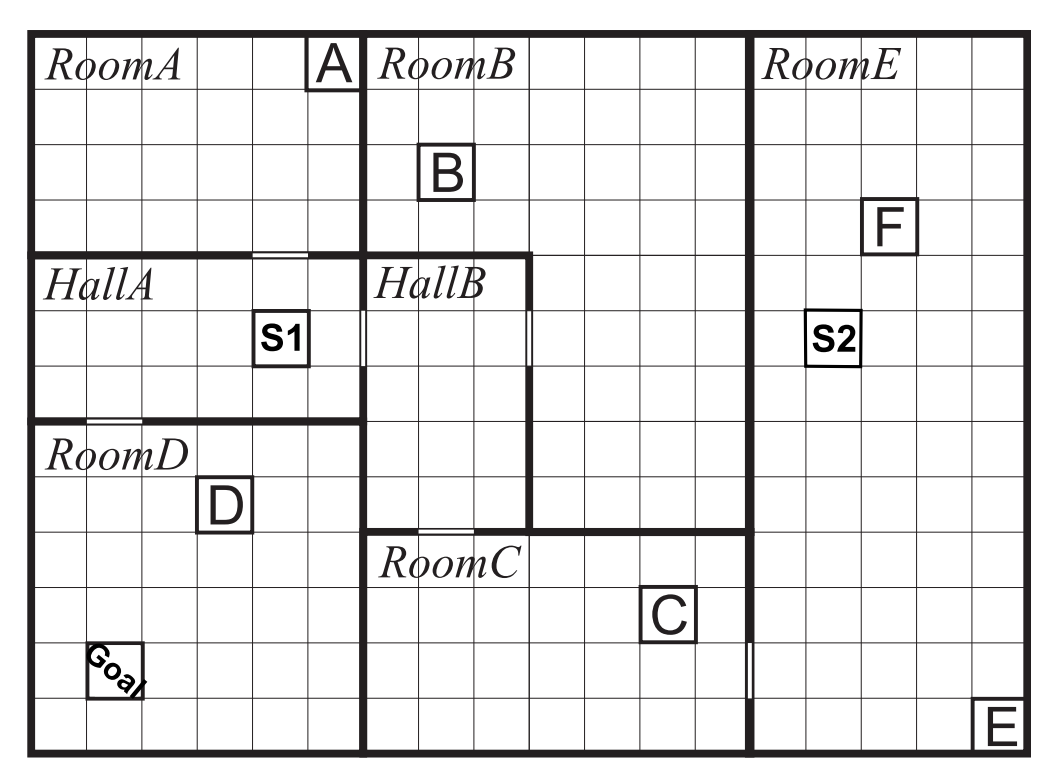
\includegraphics[width=\linewidth]{../article/img/stydyCase.png}
  \caption{Multi-Agent, Flag-Collecting Problem Domain.}
  \label{fig:studycase1}
\end{figure}
\end{column}

\begin{column}{0.5\linewidth}
\begin{block}{}
\begin{itemize}
\item Two agents
\item Six flags
\item Seven rooms
\item One goal
\item Reward  $\left\{
\begin{array}{l}
on\ goal =  Flags*100 \\
not\ on\ goal = 0
\end{array}
\right.$
\end{itemize}


\end{block}
\end{column}

\end{columns}

\end{frame}
\begin{frame}{Potential Function}
\begin{figure}[h!]
\centering
  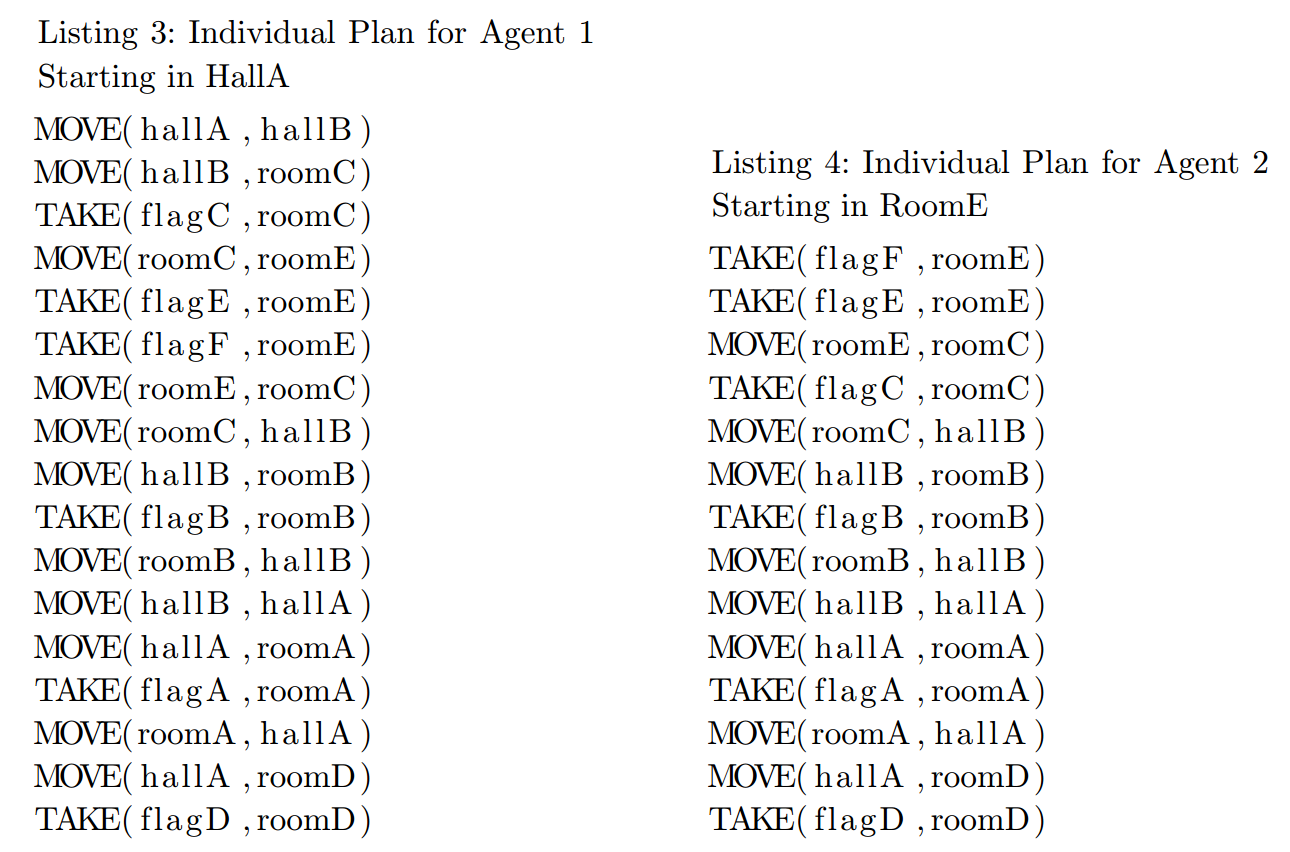
\includegraphics[height = 0.2\textheight]{../article/img/individualPlan.png}
  \caption{Individual plan.}
  \label{fig:plan1}
\end{figure}

\begin{figure}[h!]
\centering
  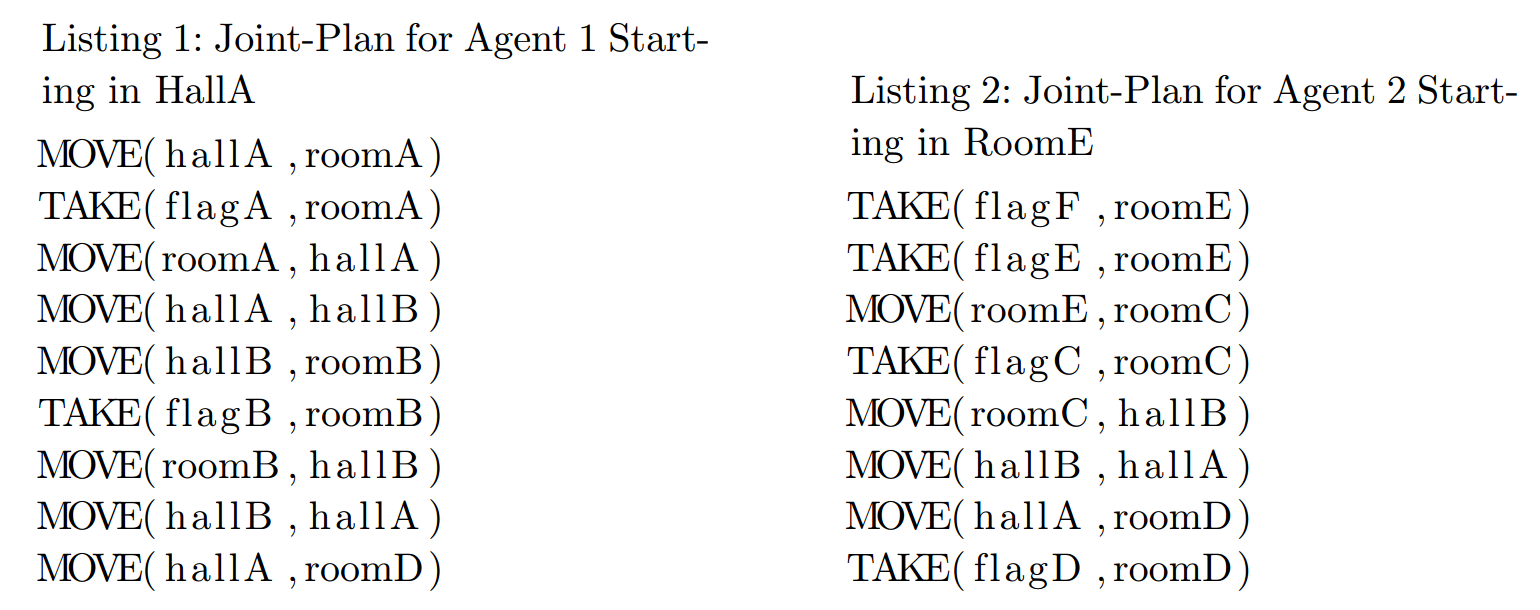
\includegraphics[height = 0.2\textheight]{../article/img/joinPlan.png}
  \caption{Joint plan.}
  \label{fig:plan2}
\end{figure}

\begin{block}{}
\begin{itemize}
\item 
\end{itemize}
\end{block}

\end{frame}

\begin{frame}{Other Heuristics}

\begin{block}{Flag-Based}
\begin{itemize}
\item $\phi (s) =  NumFlagsCollected*\omega$
\item $\omega = MaxReward/MaxFlagsInWorld$
\end{itemize}
\end{block}

\begin{block}{Flag-Based and Plan-Based}
\begin{itemize}
\item $\phi (s) = \omega * (CurrentStepInPlan + NumFlagsCollected)$
\item $\omega = MaxReward/(NumStepsInPlan + NumFlagsInWorld)$
\end{itemize}
\end{block}

\end{frame}


\section{Results and Discussion}

\subsection{Initial Results}
\begin{frame}{Initial Results}

\begin{figure}[h!]
  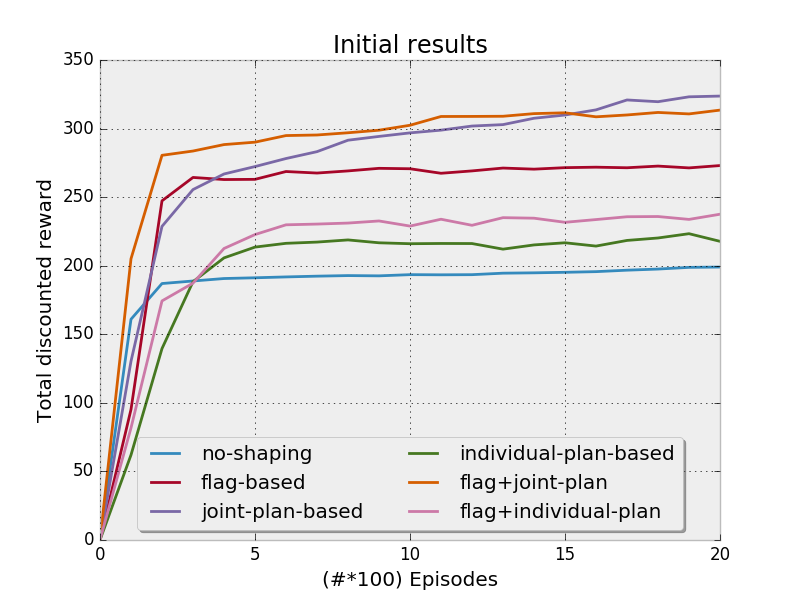
\includegraphics[height=0.4\textheight]{../article/img/initial.png}
  \caption{Initial results.}
  \label{fig:results1}
\end{figure}

\begin{block}{}
\begin{itemize}
\item 
\end{itemize}
\end{block}

\end{frame}

\begin{frame}{Conflict Knowledge}

\begin{figure}[h!]
  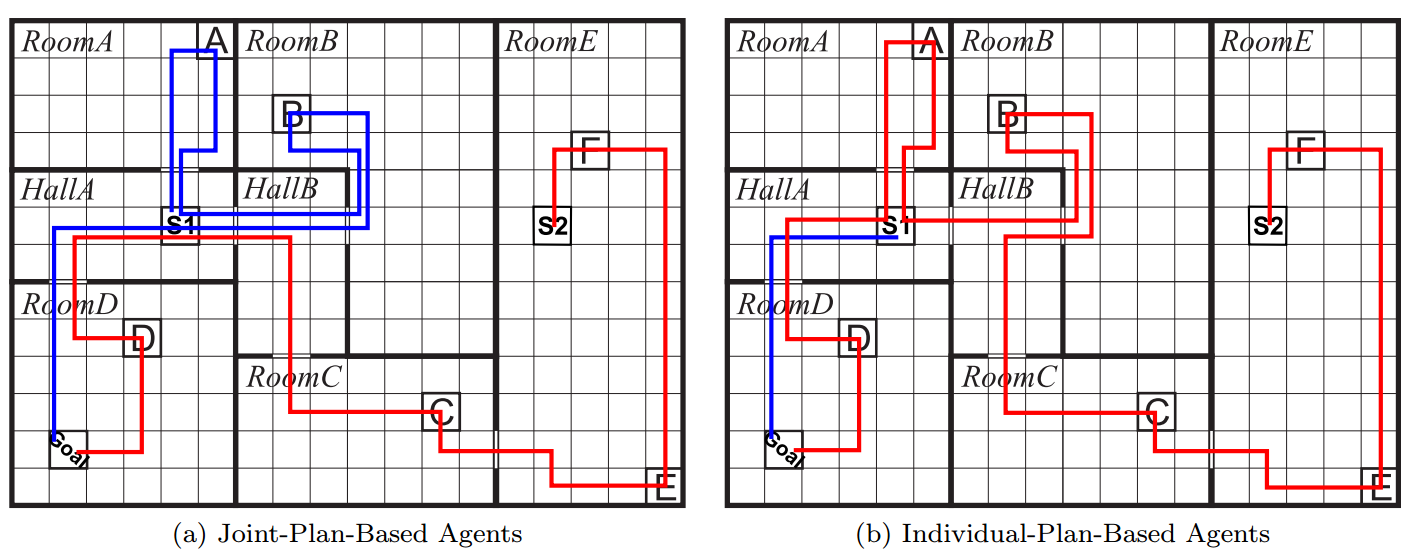
\includegraphics[height=0.4\textheight]{../article/img/behavious.png}
  \caption{Behaviours of :}
  \label{fig:behave}
\end{figure}

\end{frame}

\subsection{Improved Knowledge}
\begin{frame}{Improved Knowledge}


\begin{figure}[h!]
  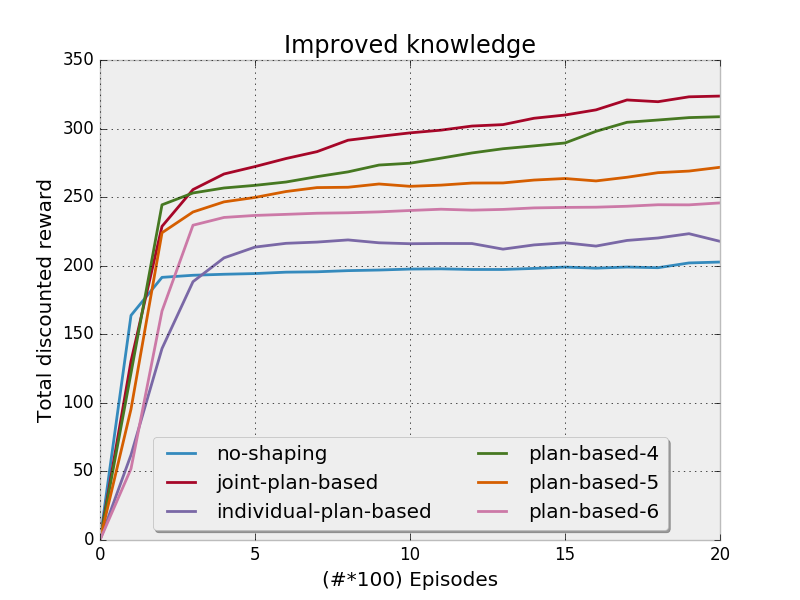
\includegraphics[height=0.4\textheight]{../article/img/knowledge.png}
  \caption{Improved knowledge.}
  \label{fig:results2}
\end{figure}

\begin{block}{}
\begin{itemize}
\item 
\end{itemize}
\end{block}

\end{frame}

\subsection{Improved Cooperation}
\begin{frame}{Improved Cooperation}


\begin{figure}[h!]
  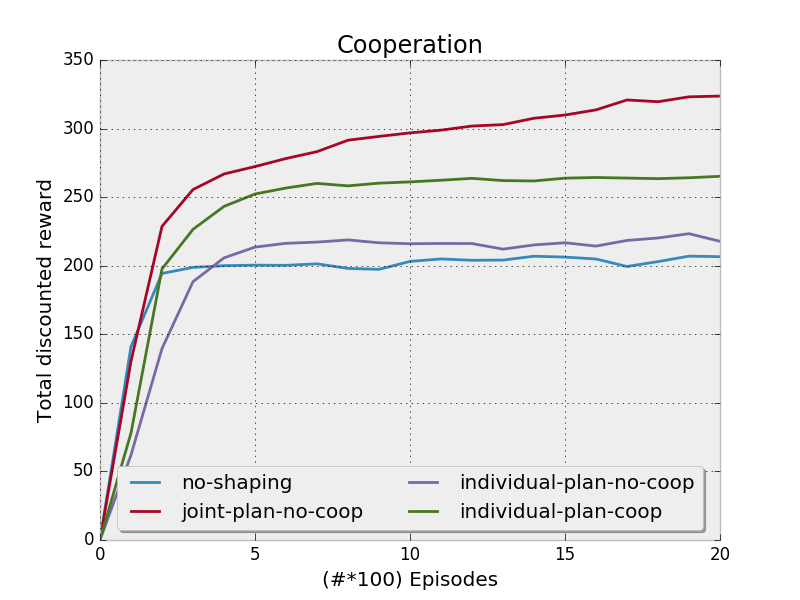
\includegraphics[height=0.4\textheight]{../article/img/coop.png}
  \caption{Improved knowledge.}
  \label{fig:results2}
\end{figure}

\begin{block}{}
\begin{itemize}
\item 
\end{itemize}
\end{block}

\end{frame}


\section{Conclusion}

\subsection{Discussion}
\begin{frame}{Discussion}

\begin{block}{}
\begin{itemize}
\item 
\end{itemize}
\end{block}

\end{frame}

\subsection{Future Work}
\begin{frame}{Future Work}

\begin{block}{}
\begin{itemize}
\item 
\end{itemize}
\end{block}

\end{frame}


\end{document}